\subsubsection{Typ}
Java-klass
\subsubsection{Syfte}
Att ta skärmdumpar och skapa en JSON-fil med information om när dessa togs.
Se URD-krav 3.1.1
\subsubsection{Funktionalitet}
Klassen har publika funktioner för att starta och avsluta inspelning. Vid inspelning används basaktiviteten för att ta reda på vilken aktivitet som användaren befinner sig i. Skärmdumpar tas sedan från aktivitetens vyer så ofta som det är möjligt. Samtidigt sparas tiden mellan varje skärmdump. När inspelningen avslutas sparas tidsinformationen ner i en JSON-fil och alla bilder i ett komprimerat format. 

\subsubsection{Underordnade komponenter}
Inga underordnade komponenter
\subsubsection{Beroenden}
Skärminspelningskomponenten beror på basaktiviteten som ger oss möjlighet att veta vilken aktivitet som användaren befinner sig i.
\subsubsection{Gränssnitt}

\subsubsection{Resurser}
Förutom redan nämnt beroende krävs tillgång till Androids SDK. Kräver också utrymme för skärmdumparna.
\subsubsection{Referenser}

\subsubsection{Process}
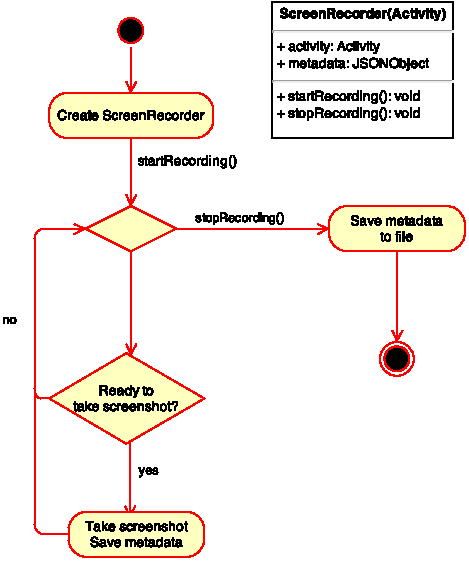
\includegraphics[scale=1.0]{screenflow.pdf}
\subsubsection{Data}
Bilderna komprimeras till PNG. JSON-filen med metadata ser ut som nedan.

\begin{verbatim}
{
   "startTime": 1393793372495,
   "timestamps": [ 307, 310, 361, ... ,352, 344 ]
}
\end{verbatim}